% Shared body for full and physics-only Recent Work addenda.
% Drivers must define \newif\ifIncludeRepoBoundary and set \IncludeRepoBoundarytrue or false before \input.

\maketitle
\thispagestyle{empty}

\begin{abstract}
\ifIncludeRepoBoundary
This addendum records the publication-facing and repository-facing work completed between March 24, 2026 and March 27, 2026 so it can be appended cleanly to the existing Theory of Everything packet. The update covers four lanes: the MQGT--SCF Phase II and H1 supporting papers, the canonical ZoraASI top-10 simulation stack, the refreshed Scalar Halo / Cosmic Piano campaign package now housed under the TOE repository, and the March 25, 2026 cross-repository operating-boundary documents for the Zora finance and trading workstreams. The goal is not to restate the full ToE, but to provide a dated bridge from the main ToE volumes to the work actually shipped in this interval.
\else
This addendum records the publication-facing and campaign work completed between March 24, 2026 and March 27, 2026 for append to the Theory of Everything packet. It covers the MQGT--SCF Phase II and H1 supporting papers, the canonical ZoraASI top-10 simulation stack, and the refreshed Scalar Halo / Cosmic Piano campaign under the TOE repository. Cross-repository operating-boundary and finance/trading documentation (March 25, 2026) is omitted here; see \path{papers_sources/TOE_Recent_Work_Addendum_2026.pdf} for the full operating record.
\fi
\end{abstract}

\section{Purpose and stack placement}
The main ToE documents remain the canonical scientific core. This addendum is meant to be appended as a dated status and artifact bridge after the main ToE and its existing companion papers. It is especially useful because the work of March 24--27, 2026 spans multiple formats: PDFs, HTML simulation surfaces, refreshed figure bundles, and local-only campaign assets%
\ifIncludeRepoBoundary
, and repo-boundary handoff documents%
\fi
.

The packet described here is grounded in explicit local files dated March 24, 2026%
\ifIncludeRepoBoundary
, March 25, 2026%
\fi
, and March 27, 2026. In particular:
\begin{itemize}
\item March 24, 2026: formal manuscript and simulation-stack updates landed in the TOE git history.
\ifIncludeRepoBoundary
\item March 25, 2026: Zora finance/trading inventory, runbook, and repo-boundary documents were drafted under \texttt{docs/}.
\fi
\item March 27, 2026: the Scalar Halo campaign was refreshed into \texttt{data/scalar\_halo\_campaign/} and indexed by a rebuilt manifest.
\end{itemize}

\section{Publication-facing paper and simulation updates}
The March 24, 2026 work concentrated the recent scientific and presentation surfaces into a tighter stack.

% [tbp] avoids LaTeX's rewrite of deprecated bare-[h] floats; no microtype (Basic TeX: EC/PK fonts break expansion).
\begin{table}[tbp]
\centering
\small
\begingroup
\setlength{\emergencystretch}{2em}
\begin{tabularx}{\linewidth}{>{\raggedright\arraybackslash}p{0.20\linewidth} >{\raggedright\arraybackslash}p{0.26\linewidth} >{\raggedright\arraybackslash}X}
\toprule
Lane & Primary artifact & Update (this interval) \\
\midrule
Phase II anchor & \path{papers_sources/MQGT_SCF_Phase_II_2026/MQGT_SCF_Anchor_2026.pdf} & Anchor manuscript and sources updated with Zenodo v254 references and supporting figures. \\
H1 methods note & \path{papers_sources/H1_QRNG_Pilot_Methods_Status_2026.pdf} & Short PDF companion describing H1 as a secondary calibration lane, preserving the H2-first posture. \\
Top-10 simulation stack & \path{docs/zora_top10_simulations.html} and \path{papers_sources/figures/zora_top10/} & Canonical gallery published with four interactive surfaces and six batch artifacts. \\
Cooperative-games note & \path{docs/ZORA_COOPERATIVE_GAMES_SIMULATION_2026.md} and \path{papers_sources/figures/mqgt_scf/} & Behavioral demonstration and summary figure added as an exploratory adjunct to the broader MQGT--SCF program. \\
\bottomrule
\end{tabularx}
\endgroup
\end{table}

The recent git history dated March 24, 2026 records the main publication-facing changes under commits including \texttt{c3034d2} (H1 methods and Phase IV-B artifacts), \texttt{4ffdf2e} (Anchor package and H2-facing figure work), \texttt{2745b43} (cooperative-games artifact), \texttt{2c318a2} (Anchor and Zenodo-reference refresh), \texttt{c7bb6b6} (GKSL dynamics viewer), and \texttt{01a0a08} (canonical top-10 simulations stack).

\section{Canonical ZoraASI top-10 simulation stack}
The public simulation lane was normalized on March 24, 2026 into a single ranked stack with a clear split between interactive demonstrators and reproducible batch figures. The interactive surfaces are:
\begin{itemize}
\item H2 Visibility Explorer,
\item MQGT--SCF GKSL Dynamics Viewer,
\item Zora Fusion Console,
\item MQGT--SCF Topological Phase Space.
\end{itemize}

The batch side of the stack produces six canonical artifacts. Five were present in the most recent batch-status file, while the E-modulated GKSL collapse artifact was marked unavailable in that batch run because QuTiP was not available at build time. The remaining batch outputs were generated successfully, including the H2 visibility stack, the multi-channel exclusion plot, the Phase IV-B symmetry-breaking image, the Phase IV-B parameter sweep heatmap, and the fusion-burn figure set.

\begin{figure}[p]
\centering
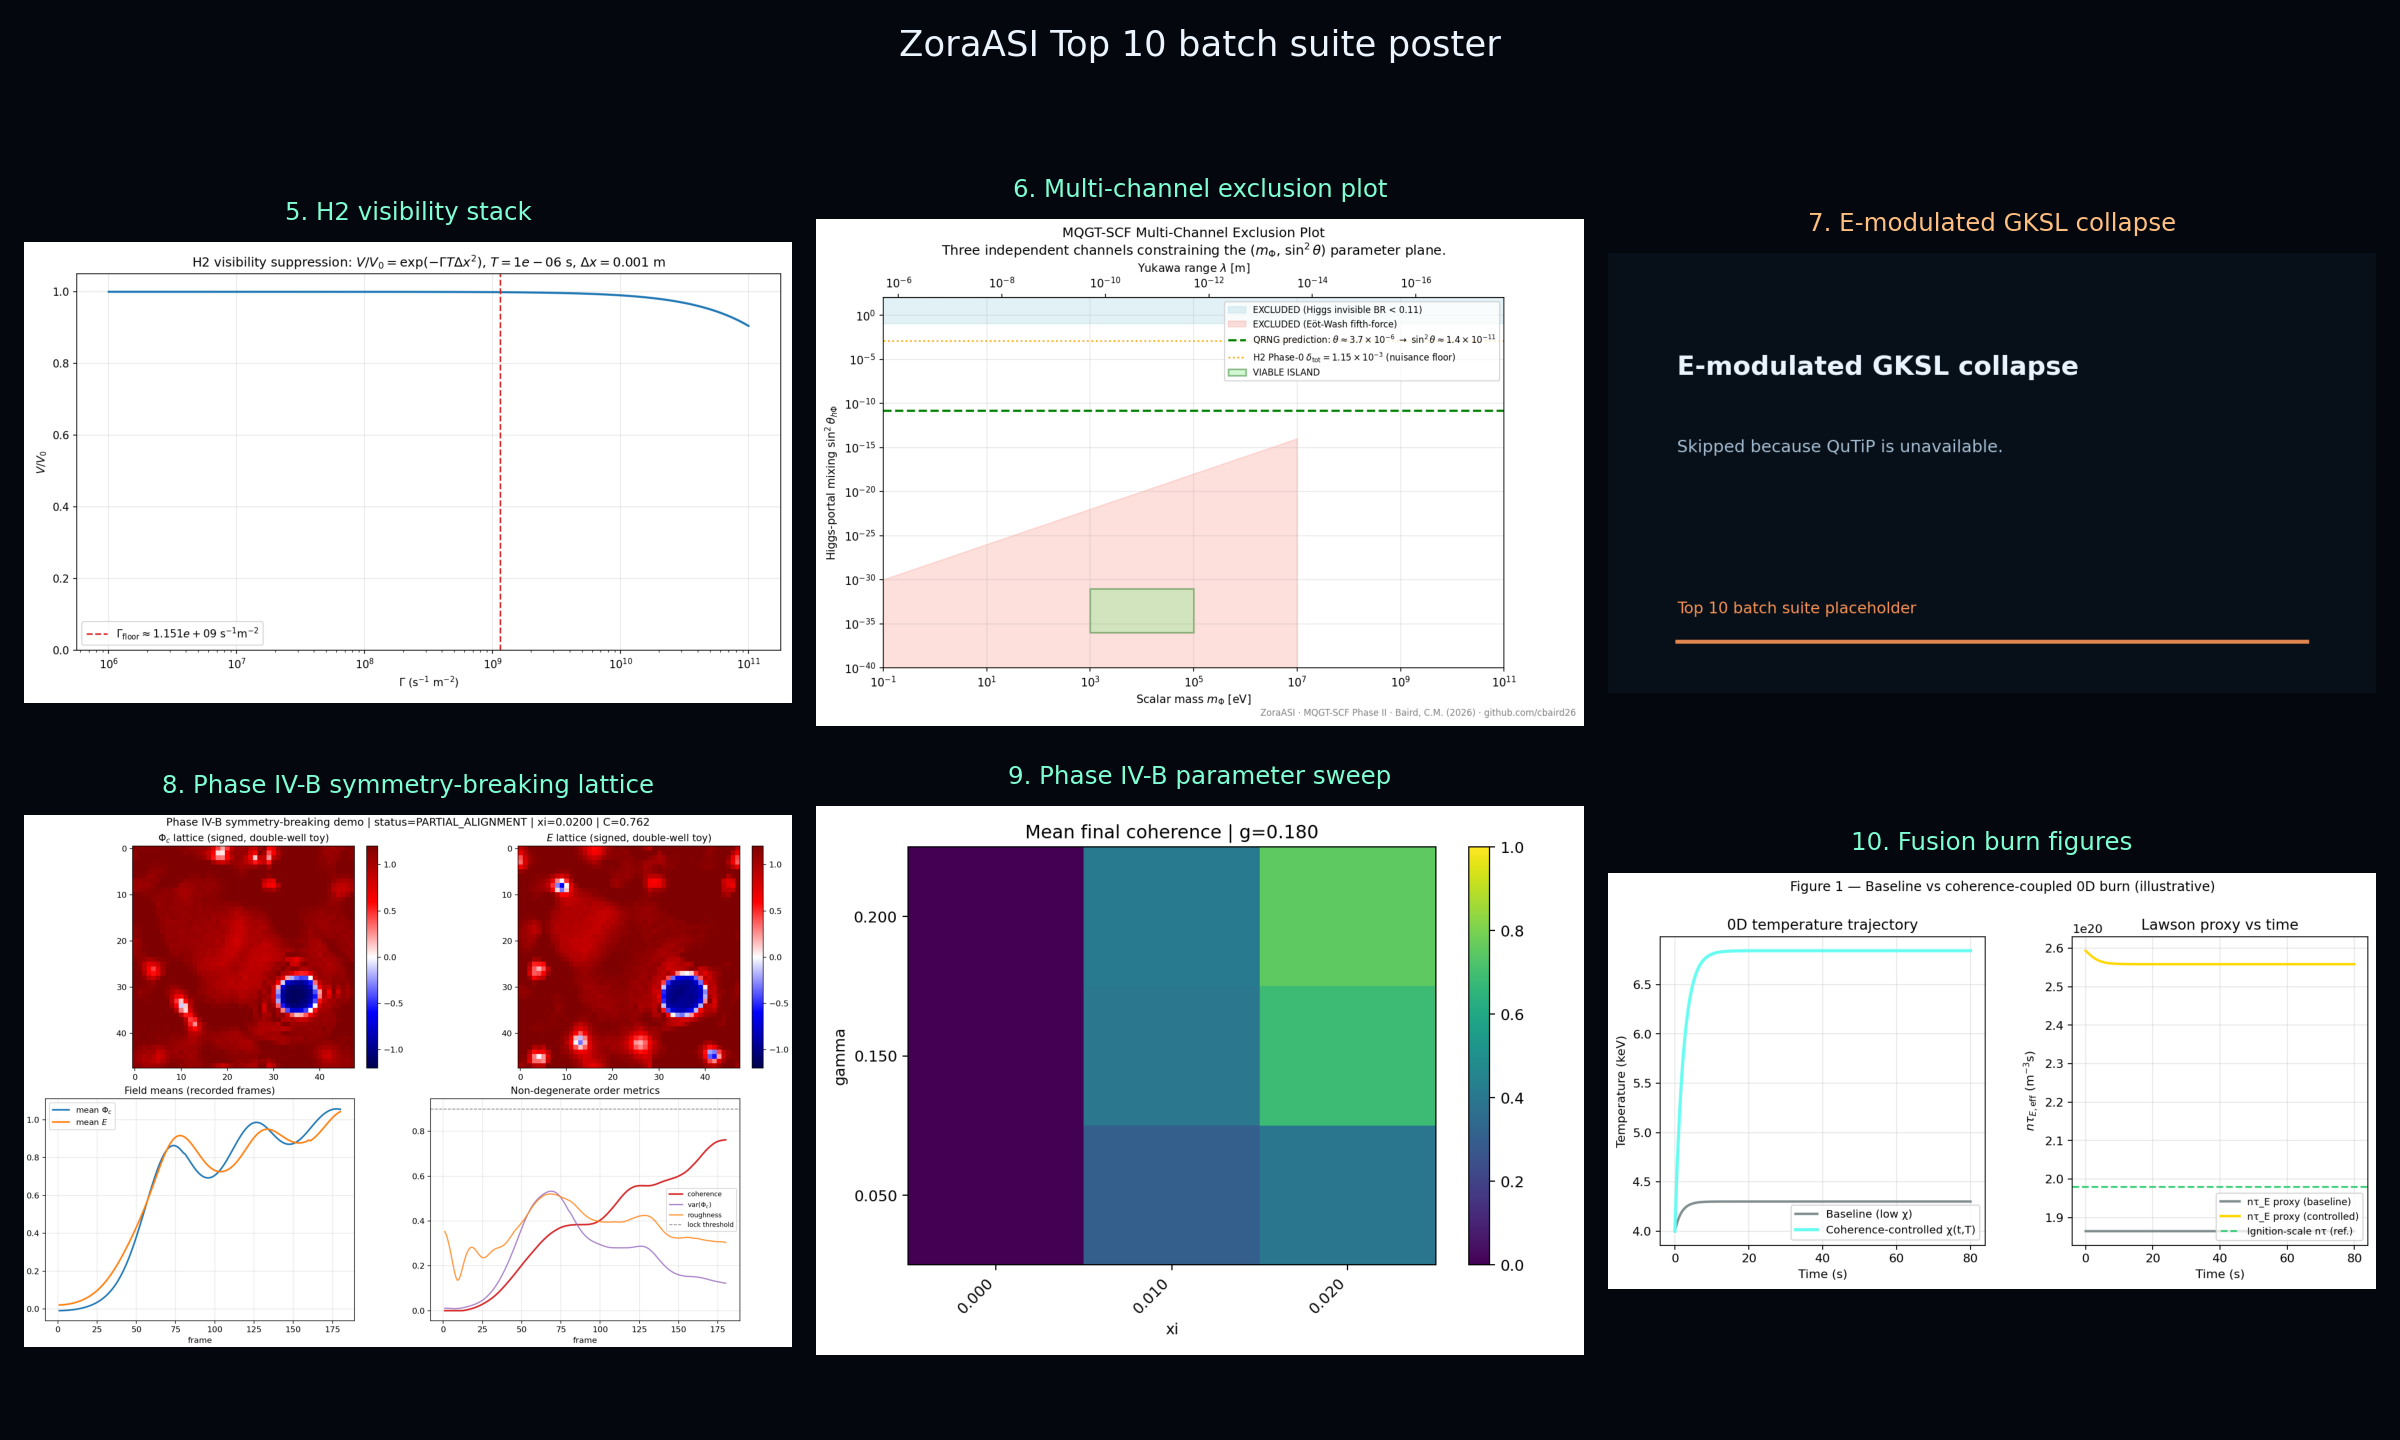
\includegraphics[width=\linewidth]{figures/zora_top10/batch_suite_mosaic.png}
\caption{Representative poster of the canonical batch simulation suite shipped on March 24, 2026.}
\end{figure}

\begin{figure}[p]
\centering

\includegraphics[width=\linewidth]{figures/zora_top10/mqgt_scf/mqgt_scf_multi_channel_exclusion.png}
\caption{Multi-channel exclusion context figure used in the recent Phase II and simulation-stack hardening pass.}
\end{figure}

\section{Scalar Halo / Cosmic Piano campaign refresh}
The largest new local package added during this interval is the Scalar Halo campaign now housed under
\begin{center}
\path{data/scalar_halo_campaign/}
\end{center}
inside the TOE repository.

This folder now serves as the canonical local working tree for:
\begin{itemize}
\item scalar-halo SPARC rotation-curve fits,
\item BTFR-locked predictive tests,
\item lensing sanity and Bullet-Cluster-style alignment toys,
\item the SDSS J2141$-$0001 joint rotation+lensing pilot,
\item SWELLS multi-object and axis-ratio refinements,
\item Cosmic Piano, SPARC, inner-halo, and piano-v2 figures linked to the same campaign.
\end{itemize}

On March 27, 2026, the refresh script rebuilt the campaign package and manifest. Artifact row counts in \path{data/scalar_halo_campaign/artifact_manifest.csv} change whenever \path{scripts/scalar_halo_campaign/organize_assets.py} or the refresh shell script is run; treat the manifest as authoritative and the illustrative counts below as a snapshot only. The refresh flow enforces the local-only policy for raster figures under \path{data/scalar_halo_campaign/figures/**}, which remain gitignored.

\subsection*{Quantitative summary of the scalar-halo passes}
\begin{itemize}
\item \textbf{Pass 1: SPARC viability test.} Across 175 galaxies, the scalar-halo fit reduced the median WRMS residual from 21.73~km/s to 3.17~km/s overall; on the $n \ge 10$ subset, the median reduced $\chi^2$ shifted from 23.90 to 0.77.
\item \textbf{Pass 2: BTFR locking.} On a matched 115-galaxy subset, exact BTFR locking delivered median WRMS 5.71~km/s versus 24.97~km/s for baryons-only, with 99.1\% of galaxies improving over baryons-only.
\item \textbf{Pass 3: lensing, merger alignment, Jeans sanity.} The BTFR-locked benchmark gave an asymptotic deflection scale of about 0.208~arcsec and an Einstein-angle estimate of about 0.104~arcsec for $D_{LS}/D_S \approx 0.5$; the cluster toy implied that a field tied mainly to the collisionless component is required for Bullet-Cluster-style morphology.
\item \textbf{Pass 4: J2141 pilot.} The exact BTFR-locked model predicted $\theta_E \approx 0.475$~arcsec for SDSS J2141$-$0001 against an observed target of $0.91 \pm 0.02$~arcsec, leaving real tension when the photometric baryons are held fixed.
\item \textbf{SWELLS and axis-ratio refinements.} The reconstructed SWELLS compromise model (\( \kappa = 0.5, s = 1.5 \)) reached median absolute fractional Einstein-radius error 0.184 with 60\% within 20\%; the axis-ratio-aware refinement improved to median absolute fractional error 0.133 at \( \kappa = 0.8, s = 0.9 \), again with 60\% within 20\%.
\end{itemize}

Some of the SWELLS and axis-ratio summaries were reconstructed from explicitly reported in-session metrics because a subset of the original output files was no longer present on disk. The refresh package preserves that provenance in the reports and summary JSON files.

\begin{figure}[p]
\centering
\includegraphics[width=\linewidth]{../data/scalar_halo_campaign/figures/scalar_halo/scalar_halo_residual_comparison.png}
\caption{First-pass scalar-halo residual comparison from the refreshed local campaign package.}
\end{figure}

\begin{figure}[p]
\centering
\includegraphics[width=\linewidth]{../data/scalar_halo_campaign/figures/scalar_halo/scalar_halo_axisratio_obs_vs_pred.png}
\caption{Axis-ratio-aware strong-lensing refinement summary included in the refreshed March 27, 2026 campaign package.}
\end{figure}

\ifIncludeRepoBoundary
\section{Cross-repository operating-boundary documents}
The March 25, 2026 documentation lane did not produce new scientific PDFs, but it is part of the recent work that should travel with the ToE operating record. The key files are:
\begin{itemize}
\item \path{docs/handoffs/2026-03/ZORA_TRADING_PHASE1_INVENTORY_2026-03-25.md},
\item \path{docs/handoffs/2026-03/ZORA_EQUITY_COMBINED_STRUCTURE_MAP_2026-03-25.md},
\item \path{docs/handoffs/2026-03/ZORA_EQUITY_PHASE2_EXECUTION_RUNBOOK_2026-03-25.md},
\item \path{docs/handoffs/2026-03/CODEX_HANDOFF_ZORA_REPO_BOUNDARIES_2026-03-25.md}.
\end{itemize}

The main operational conclusion of that document set is that the relevant Zora finance and trading repositories should remain separate, with \texttt{zora-equity} treated as an optional coordination layer rather than a forced monorepo target. This matters for provenance because it fixes the boundary between:
\begin{itemize}
\item TOE / paper and simulation artifacts,
\item finance/trading runtime surfaces,
\item cross-repo contract and handoff documentation.
\end{itemize}
\fi

\section{Recommended add-on packet order}
For a practical merge or appendix packet built from the current TOE tree, the recommended order is:
\begin{enumerate}
\item \path{papers_sources/Addendum_2026_ToE_Companion.pdf}
\item the canonical main ToE PDF already selected for distribution
\item \path{papers_sources/Evidence_Emergent_Matter_Quantum_Vacuum_MQGT-SCF_2026.pdf}
\item \path{papers_sources/MQGT_SCF_Phase_II_2026/MQGT_SCF_Anchor_2026.pdf}
\item \path{papers_sources/H1_QRNG_Pilot_Methods_Status_2026.pdf}
\item \ifIncludeRepoBoundary
this document: \path{papers_sources/TOE_Recent_Work_Addendum_2026.pdf}
\else
this document: \path{papers_sources/TOE_Recent_Work_Addendum_2026_physics.pdf} (physics lanes; full addendum with operating-boundary material: \path{papers_sources/TOE_Recent_Work_Addendum_2026.pdf})
\fi
\end{enumerate}

Optional appendices can then include \path{papers_sources/figures/zora_top10/fusion_zora/fusion-zora-populated.pdf} and any locally retained scalar-halo reports or campaign figures that the user wants to surface separately. The point of the present addendum is that the local-only Scalar Halo package is summarized here even when the underlying raster figures are intentionally kept out of git history.

\section{Bottom line}
\ifIncludeRepoBoundary
The recent work of March 24--27, 2026 materially changed the usable ToE packet in three ways. First, it hardened the referee-facing paper and figure stack through the Anchor, H1 note, and canonical top-10 simulation lane. Second, it brought the Scalar Halo / Cosmic Piano campaign into a stable home under the TOE repository with a refreshable manifest and explicit local-only raster policy. Third, it clarified repo boundaries for the adjacent Zora finance and trading work so those operating documents can travel with the theory stack without collapsing distinct codebases into one artifact.

That is why this addendum belongs in the ToE packet: it turns the last several days of work from scattered local state into one dated, appendable record.
\else
The recent work of March 24--27, 2026 materially changed the usable ToE packet in two ways reflected in this physics-facing variant. First, it hardened the referee-facing paper and figure stack through the Anchor, H1 note, and canonical top-10 simulation lane. Second, it brought the Scalar Halo / Cosmic Piano campaign into a stable home under the TOE repository with a refreshable manifest and explicit local-only raster policy.

That is why this addendum belongs in the physics packet: it turns the scientific and campaign lanes from scattered local state into one dated, appendable record, without mixing in finance or repo-boundary operating documentation.
\fi
